\documentclass{article}\usepackage[]{graphicx}\usepackage[]{xcolor}
% maxwidth is the original width if it is less than linewidth
% otherwise use linewidth (to make sure the graphics do not exceed the margin)
\makeatletter
\def\maxwidth{ %
  \ifdim\Gin@nat@width>\linewidth
    \linewidth
  \else
    \Gin@nat@width
  \fi
}
\makeatother

\definecolor{fgcolor}{rgb}{0.345, 0.345, 0.345}
\newcommand{\hlnum}[1]{\textcolor[rgb]{0.686,0.059,0.569}{#1}}%
\newcommand{\hlsng}[1]{\textcolor[rgb]{0.192,0.494,0.8}{#1}}%
\newcommand{\hlcom}[1]{\textcolor[rgb]{0.678,0.584,0.686}{\textit{#1}}}%
\newcommand{\hlopt}[1]{\textcolor[rgb]{0,0,0}{#1}}%
\newcommand{\hldef}[1]{\textcolor[rgb]{0.345,0.345,0.345}{#1}}%
\newcommand{\hlkwa}[1]{\textcolor[rgb]{0.161,0.373,0.58}{\textbf{#1}}}%
\newcommand{\hlkwb}[1]{\textcolor[rgb]{0.69,0.353,0.396}{#1}}%
\newcommand{\hlkwc}[1]{\textcolor[rgb]{0.333,0.667,0.333}{#1}}%
\newcommand{\hlkwd}[1]{\textcolor[rgb]{0.737,0.353,0.396}{\textbf{#1}}}%
\let\hlipl\hlkwb

\usepackage{framed}
\makeatletter
\newenvironment{kframe}{%
 \def\at@end@of@kframe{}%
 \ifinner\ifhmode%
  \def\at@end@of@kframe{\end{minipage}}%
  \begin{minipage}{\columnwidth}%
 \fi\fi%
 \def\FrameCommand##1{\hskip\@totalleftmargin \hskip-\fboxsep
 \colorbox{shadecolor}{##1}\hskip-\fboxsep
     % There is no \\@totalrightmargin, so:
     \hskip-\linewidth \hskip-\@totalleftmargin \hskip\columnwidth}%
 \MakeFramed {\advance\hsize-\width
   \@totalleftmargin\z@ \linewidth\hsize
   \@setminipage}}%
 {\par\unskip\endMakeFramed%
 \at@end@of@kframe}
\makeatother

\definecolor{shadecolor}{rgb}{.97, .97, .97}
\definecolor{messagecolor}{rgb}{0, 0, 0}
\definecolor{warningcolor}{rgb}{1, 0, 1}
\definecolor{errorcolor}{rgb}{1, 0, 0}
\newenvironment{knitrout}{}{} % an empty environment to be redefined in TeX

\usepackage{alltt}
\usepackage[margin=1.0in]{geometry} % To set margins
\usepackage{amsmath}  % This allows me to use the align functionality.
                      % If you find yourself trying to replicate
                      % something you found online, ensure you're
                      % loading the necessary packages!
\usepackage{amsfonts} % Math font
\usepackage{fancyvrb}
\usepackage{hyperref} % For including hyperlinks
\usepackage[shortlabels]{enumitem}% For enumerated lists with labels specified
                                  % We had to run tlmgr_install("enumitem") in R
\usepackage{float}    % For telling R where to put a table/figure
\usepackage{natbib}        %For the bibliography
\bibliographystyle{apalike}%For the bibliography
\IfFileExists{upquote.sty}{\usepackage{upquote}}{}
\begin{document}
\begin{enumerate}
%%%%%%%%%%%%%%%%%%%%%%%%%%%%%%%%%%%%%%%%%%%%%%%%%%%%%%%%%%%%%%%%%%%%%%%%%%%%%%%%
%%%%%%%%%%%%%%%%%%%%%%%%%%%%%%%%%%%%%%%%%%%%%%%%%%%%%%%%%%%%%%%%%%%%%%%%%%%%%%%%
% QUESTION 1
%%%%%%%%%%%%%%%%%%%%%%%%%%%%%%%%%%%%%%%%%%%%%%%%%%%%%%%%%%%%%%%%%%%%%%%%%%%%%%%%
%%%%%%%%%%%%%%%%%%%%%%%%%%%%%%%%%%%%%%%%%%%%%%%%%%%%%%%%%%%%%%%%%%%%%%%%%%%%%%%%
\item In Lab 3, you wrangled data from Essentia, Essentia models and LIWC. Rework your 
solution to Lab 3 using \texttt{tidyverse} \citep{tidyverse} instead of base \texttt{R}.
Specifically, rewrite your code for steps 1-4 of task 2 using \texttt{tidyverse} \citep{tidyverse}. 
Make sure to address any issues I noted in your code file, and ensure that your code 
runs in the directory as it is set up.
\begin{knitrout}\scriptsize
\definecolor{shadecolor}{rgb}{0.969, 0.969, 0.969}\color{fgcolor}\begin{kframe}
\begin{alltt}
\hlcom{# Henry Sun }
\hlcom{# Homework 5 }
\hlcom{# 2/26/25}


\hlcom{# Step 0}
\hlkwd{library}\hldef{(}\hlsng{"stringr"}\hldef{)}
\hlkwd{library}\hldef{(}\hlsng{"jsonlite"}\hldef{)}
\hlkwd{library}\hldef{(tidyverse)}


\hlcom{#Step 1, Front Bottoms Example}
\hldef{current.filename} \hlkwb{=} \hlsng{"The Front Bottoms-Talon of the Hawk-Au Revoir (Adios).json"}
\hldef{currentfile.split} \hlkwb{=} \hlkwd{str_split_1}\hldef{(current.filename,} \hlsng{"-"}\hldef{)}

\hlcom{# artist, album, track}
\hldef{artist} \hlkwb{=} \hldef{currentfile.split[}\hlnum{1}\hldef{]}
\hldef{album} \hlkwb{=} \hldef{currentfile.split[}\hlnum{2}\hldef{]}
\hldef{track} \hlkwb{=} \hlkwd{str_sub}\hldef{(currentfile.split[}\hlnum{3}\hldef{],} \hlkwc{start} \hldef{=} \hlnum{0}\hldef{,} \hlkwc{end} \hldef{=} \hlopt{-}\hlnum{6}\hldef{)}

\hlcom{# Essentia Output}
\hldef{curr.json} \hlkwb{=} \hldef{(}\hlkwd{fromJSON}\hldef{(}\hlkwd{paste}\hldef{(}\hlsng{"EssentiaOutput/"}\hldef{, current.filename,} \hlkwc{sep}\hldef{=}\hlsng{""}\hldef{)))}

\hlcom{# lowlevel}
\hldef{overall.loudness} \hlkwb{=} \hldef{curr.json}\hlopt{$}\hldef{lowlevel}\hlopt{$}\hldef{loudness_ebu128}\hlopt{$}\hldef{integrated}
\hldef{spectral.energy} \hlkwb{=} \hldef{curr.json}\hlopt{$}\hldef{lowlevel}\hlopt{$}\hldef{spectral_energy}\hlopt{$}\hldef{mean}
\hldef{dissonance} \hlkwb{=} \hldef{curr.json}\hlopt{$}\hldef{lowlevel}\hlopt{$}\hldef{dissonance}\hlopt{$}\hldef{mean}
\hldef{pitch.salience} \hlkwb{=} \hldef{curr.json}\hlopt{$}\hldef{lowlevel}\hlopt{$}\hldef{pitch_salience}\hlopt{$}\hldef{mean}

\hlcom{# rhythm}
\hldef{bpm} \hlkwb{=} \hldef{curr.json}\hlopt{$}\hldef{rhythm}\hlopt{$}\hldef{bpm}
\hldef{beats.loudness} \hlkwb{=} \hldef{curr.json}\hlopt{$}\hldef{rhythm}\hlopt{$}\hldef{beats_loudness}\hlopt{$}\hldef{mean}
\hldef{danceability} \hlkwb{=} \hldef{curr.json}\hlopt{$}\hldef{rhythm}\hlopt{$}\hldef{danceability}

\hlcom{# tonal}
\hldef{tuning.freq} \hlkwb{=} \hldef{curr.json}\hlopt{$}\hldef{tonal}\hlopt{$}\hldef{tuning_frequency}

\hlcom{# data from example file}
\hldef{currfile.data} \hlkwb{=} \hlkwd{tibble}\hldef{(overall.loudness, spectral.energy, dissonance, pitch.salience, bpm, beats.loudness,}
                  \hldef{danceability, tuning.freq)}


\hlcom{# Step 2, repeat for all .json files}
\hlcom{# load files}
\hldef{all.files} \hlkwb{=} \hldef{(}\hlkwd{list.files}\hldef{(}\hlsng{"EssentiaOutput"}\hldef{,} \hlkwc{recursive}\hldef{=}\hlnum{TRUE}\hldef{))}

\hlcom{# only check files with .json }
\hldef{json.check} \hlkwb{=} \hlkwd{str_count}\hldef{(all.files,} \hlkwc{pattern}\hldef{=}\hlsng{".json"}\hldef{)}
\hldef{all.json} \hlkwb{=} \hldef{all.files[}\hlkwd{which}\hldef{(json.check} \hlopt{==} \hlnum{1}\hldef{)]}

\hlcom{# create tibble}
\hldef{json.data} \hlkwb{=} \hlkwd{tibble}\hldef{(}
  \hlkwc{artist} \hldef{=} \hlkwd{character}\hldef{(),}
  \hlkwc{album} \hldef{=} \hlkwd{character}\hldef{(),}
  \hlkwc{overall.loudness} \hldef{=} \hlkwd{numeric}\hldef{(),}
  \hlkwc{spectral.energy} \hldef{=} \hlkwd{numeric}\hldef{(),}
  \hlkwc{dissonance} \hldef{=} \hlkwd{numeric}\hldef{(),}
  \hlkwc{pitch.salience} \hldef{=} \hlkwd{numeric}\hldef{(),}
  \hlkwc{bpm} \hldef{=} \hlkwd{numeric}\hldef{(),}
  \hlkwc{beats.loudness} \hldef{=} \hlkwd{numeric}\hldef{(),}
  \hlkwc{danceability} \hldef{=} \hlkwd{numeric}\hldef{(),}
  \hlkwc{tuning.freq} \hldef{=} \hlkwd{numeric}\hldef{()}
\hldef{)}

\hlcom{# repeat same for all files in step 1}
\hlkwa{for} \hldef{(i} \hlkwa{in} \hlnum{1}\hlopt{:}\hlkwd{length}\hldef{(all.json))\{}
  \hldef{curr.file} \hlkwb{=} \hlkwd{fromJSON}\hldef{(}\hlkwd{paste}\hldef{(}\hlsng{"EssentiaOutput/"}\hldef{, all.json[i],} \hlkwc{sep} \hldef{=} \hlsng{""}\hldef{))}
  \hldef{currfile.split} \hlkwb{=}  \hlkwd{str_split_1}\hldef{(all.json[i],} \hlsng{"-"}\hldef{)}

  \hldef{artist} \hlkwb{=} \hldef{currfile.split[}\hlnum{1}\hldef{]}
  \hldef{album} \hlkwb{=} \hldef{currfile.split[}\hlnum{2}\hldef{]}
  \hldef{track} \hlkwb{=} \hlkwd{str_sub}\hldef{(currfile.split[}\hlnum{3}\hldef{],} \hlkwc{start} \hldef{=} \hlnum{0}\hldef{,} \hlkwc{end} \hldef{=} \hlopt{-}\hlnum{6}\hldef{)}

  \hldef{overall.loudness} \hlkwb{=} \hldef{curr.file}\hlopt{$}\hldef{lowlevel}\hlopt{$}\hldef{loudness_ebu128}\hlopt{$}\hldef{integrated}
  \hldef{spectral.energy} \hlkwb{=} \hldef{curr.file}\hlopt{$}\hldef{lowlevel}\hlopt{$}\hldef{spectral_energy}\hlopt{$}\hldef{mean}
  \hldef{dissonance} \hlkwb{=} \hldef{curr.file}\hlopt{$}\hldef{lowlevel}\hlopt{$}\hldef{dissonance}\hlopt{$}\hldef{mean}
  \hldef{pitch.salience} \hlkwb{=} \hldef{curr.file}\hlopt{$}\hldef{lowlevel}\hlopt{$}\hldef{pitch_salience}\hlopt{$}\hldef{mean}
  \hldef{bpm} \hlkwb{=} \hldef{curr.file}\hlopt{$}\hldef{rhythm}\hlopt{$}\hldef{bpm}
  \hldef{beats.loudness} \hlkwb{=} \hldef{curr.file}\hlopt{$}\hldef{rhythm}\hlopt{$}\hldef{beats_loudness}\hlopt{$}\hldef{mean}
  \hldef{danceability} \hlkwb{=} \hldef{curr.file}\hlopt{$}\hldef{rhythm}\hlopt{$}\hldef{danceability}
  \hldef{tuning.freq} \hlkwb{=} \hldef{curr.file}\hlopt{$}\hldef{tonal}\hlopt{$}\hldef{tuning_frequency}

  \hlcom{# insert into tibble}
  \hlcom{# create row of data for each song, add to tibble}
  \hldef{json.data} \hlkwb{=} \hlkwd{bind_rows}\hldef{(json.data,} \hlkwd{tibble}\hldef{(}
    \hldef{artist, album, track, overall.loudness,}
    \hldef{spectral.energy, dissonance, pitch.salience, bpm, beats.loudness,}
    \hldef{danceability, tuning.freq))}
\hldef{\}}


\hlcom{# Step 3}
\hlcom{# read csv into a tibble}
\hldef{essentia.file} \hlkwb{=} \hlkwd{read_csv}\hldef{(}\hlsng{"EssentiaOutput/EssentiaModelOutput.csv"}\hldef{)}
\hlcom{# create new cols using mutate, }
\hlcom{# use rowMeans() + cbind to find means for some features}
\hlcom{# I was trying to use bind_cols but it displayed a bunch of messages when running}
\hldef{essentia.data} \hlkwb{<-} \hldef{essentia.file |>}
  \hlkwd{mutate}\hldef{(}\hlkwc{valence} \hldef{=} \hlkwd{rowMeans}\hldef{(}\hlkwd{cbind}\hldef{(deam_valence, emo_valence, muse_valence)),}
         \hlkwc{arousal} \hldef{=} \hlkwd{rowMeans}\hldef{(}\hlkwd{cbind}\hldef{(deam_arousal, emo_arousal, muse_arousal)),}
         \hlkwc{aggressive} \hldef{=} \hlkwd{rowMeans}\hldef{(}\hlkwd{cbind}\hldef{(eff_aggressive, nn_aggressive)),}
         \hlkwc{happy} \hldef{=} \hlkwd{rowMeans}\hldef{(}\hlkwd{cbind}\hldef{(eff_happy, nn_happy)),}
         \hlkwc{party} \hldef{=} \hlkwd{rowMeans}\hldef{(}\hlkwd{cbind}\hldef{(eff_party, nn_party)),}
         \hlkwc{relaxed} \hldef{=} \hlkwd{rowMeans}\hldef{(}\hlkwd{cbind}\hldef{(eff_relax, nn_relax)),}
         \hlkwc{sad} \hldef{=} \hlkwd{rowMeans}\hldef{(}\hlkwd{cbind}\hldef{(eff_sad, nn_sad)),}
         \hlkwc{acoustic} \hldef{=} \hlkwd{rowMeans}\hldef{(}\hlkwd{cbind}\hldef{(eff_acoustic, nn_acoustic)),}
         \hlkwc{electric} \hldef{=} \hlkwd{rowMeans}\hldef{(}\hlkwd{cbind}\hldef{(eff_electronic, nn_electronic)),}
         \hlkwc{instrumental} \hldef{=} \hlkwd{rowMeans}\hldef{(}\hlkwd{cbind}\hldef{(eff_instrumental, nn_instrumental))) |>}
\hlcom{# rename timbreBright}
  \hlkwd{rename}\hldef{(}\hlkwc{timbreBright} \hldef{= eff_timbre_bright) |>}
\hlcom{# select features}
  \hlkwd{select}\hldef{(artist, album, track, valence, arousal, aggressive, happy, party, relaxed,}
         \hldef{sad, acoustic, electric, instrumental, timbreBright)}


\hlcom{# Step 4}
\hlcom{# join all data into one file, grouping by artist, album, track (eliminate dupes)}
\hldef{liwc.data} \hlkwb{=} \hlkwd{read_csv}\hldef{(}\hlsng{"LIWCOutput/LIWCOutput.csv"}\hldef{)}
\hldef{all.data} \hlkwb{<-} \hldef{essentia.data |>}
  \hlkwd{left_join}\hldef{(json.data,} \hlkwc{by} \hldef{=} \hlkwd{c}\hldef{(}\hlsng{"artist"}\hldef{,} \hlsng{"album"}\hldef{,} \hlsng{"track"}\hldef{)) |>}
  \hlkwd{left_join}\hldef{(liwc.data,} \hlkwc{by} \hldef{=} \hlkwd{c}\hldef{(}\hlsng{"artist"}\hldef{,} \hlsng{"album"}\hldef{,} \hlsng{"track"}\hldef{)) |>}
\hlcom{# rename function}
  \hlkwd{rename}\hldef{(}\hlsng{"funct"} \hldef{=} \hlsng{"function"}\hldef{)}


\hlcom{#Step 5}
\hldef{training.data} \hlkwb{=} \hlkwd{filter}\hldef{(all.data, track} \hlopt{!=} \hlsng{"Allentown"}\hldef{)}
\hldef{testing.data} \hlkwb{=} \hlkwd{filter}\hldef{(all.data, track} \hlopt{==} \hlsng{"Allentown"}\hldef{)}

\hldef{training.csv} \hlkwb{=} \hlkwd{write_csv}\hldef{(}\hlkwc{x}\hldef{=training.data,} \hlsng{"trainingdata.csv"}\hldef{)}
\hldef{testing.csv} \hlkwb{=} \hlkwd{write_csv}\hldef{(}\hlkwc{x}\hldef{=testing.data,} \hlsng{"testingdata.csv"}\hldef{)}


\hlcom{# Coding challenge, make a graph }
\hlcom{# violin plot for relaxed values}
\hldef{relaxed.plot} \hlkwb{<-} \hlkwd{ggplot}\hldef{(}\hlkwd{read_csv}\hldef{(}\hlsng{"trainingdata.csv"}\hldef{),} \hlkwd{aes}\hldef{(}\hlkwc{x}\hldef{=artist,} \hlkwc{y}\hldef{=relaxed))}\hlopt{+}
  \hlkwd{geom_violin}\hldef{(}\hlkwc{fill}\hldef{=}\hlsng{"grey80"}\hldef{)}\hlopt{+}
  \hlkwd{geom_boxplot}\hldef{(}\hlkwc{width} \hldef{=} \hlnum{0.1}\hldef{)}\hlopt{+}
  \hlkwd{geom_jitter}\hldef{(}\hlkwc{color} \hldef{=} \hlsng{"black"}\hldef{,} \hlkwc{size} \hldef{=} \hlnum{0.4}\hldef{,} \hlkwc{alpha} \hldef{=} \hlnum{0.9}\hldef{,} \hlkwc{width} \hldef{=} \hlnum{0.125}\hldef{)}\hlopt{+}
  \hlkwd{xlab}\hldef{(}\hlsng{"artist"}\hldef{)}\hlopt{+}
  \hlkwd{ylab}\hldef{(}\hlsng{"relaxed"}\hldef{)}\hlopt{+}
  \hlkwd{coord_flip}\hldef{()}
\hldef{relaxed.plot}
\end{alltt}
\end{kframe}
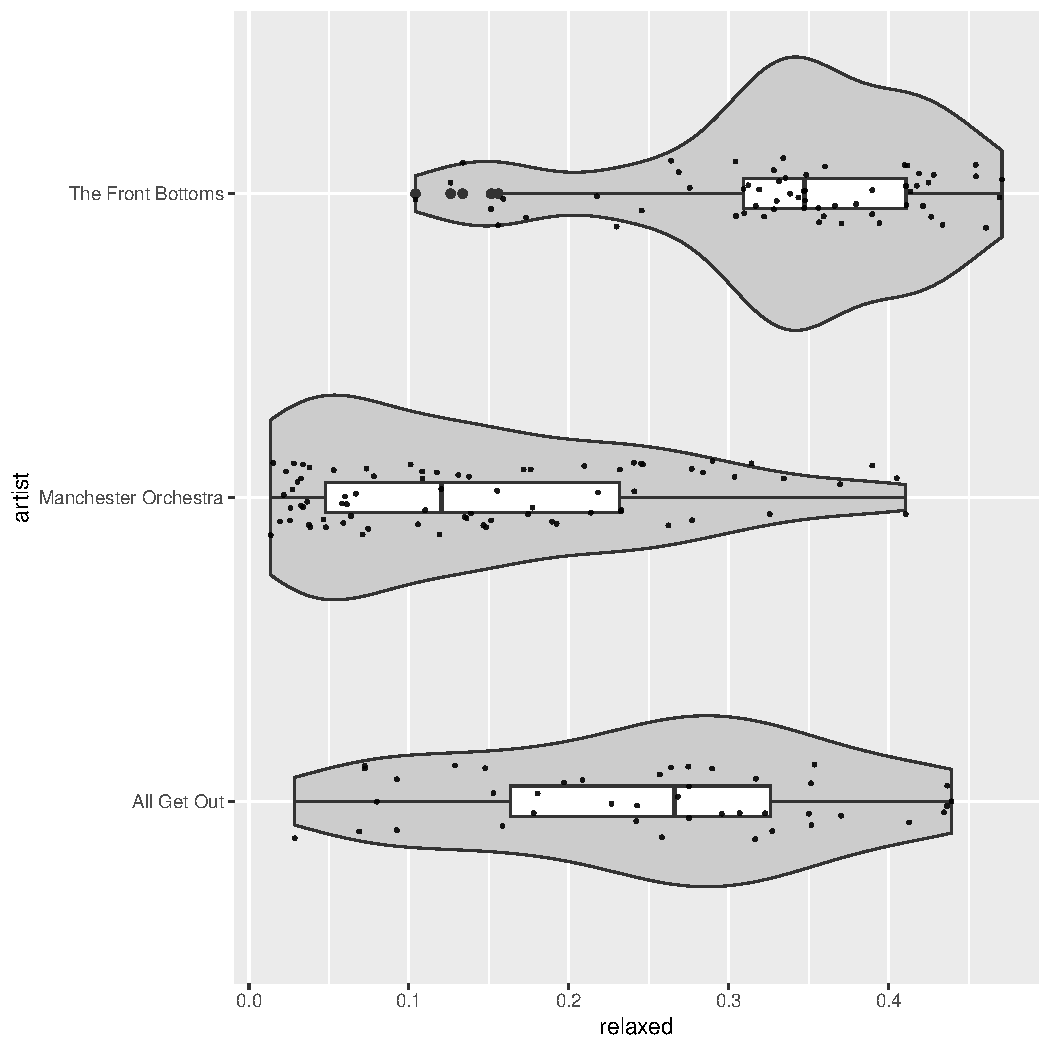
\includegraphics[width=\maxwidth]{figure/unnamed-chunk-1-1} 
\end{knitrout}
\end{enumerate}
\bibliography{bibliography}
\end{document}
